\documentclass[12pt]{standalone}
\usepackage{tikz}
%\usetikzlibrary{calc, arrows.meta, decorations.pathreplacing}

\begin{document}
	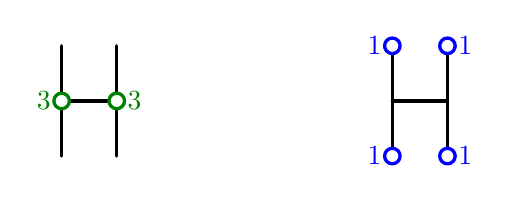
\begin{tikzpicture}[line width=1.2pt, line cap=round, line join=round, scale=1.4]

		\draw[shorten >= 3.2pt] (0,0) -- (0, 0.5);
		\draw[shorten >= 3.2pt] (0.5,0) -- (0.5, 0.5);
		\draw[shorten >= 3.2pt] (0.5,1) -- (0.5, 0.5);
		\draw[shorten >= 3.2pt] (0,1) -- (0, 0.5);
		\draw[shorten <= 3.2pt, shorten >= 3.2pt] (0,0.5) -- (0.5, 0.5);		
		\draw[green!50!black] (0, 0.5) circle(2pt) node[anchor=east]{3};
		\draw[green!50!black] (0.5, 0.5) circle(2pt) node[anchor=west]{3};
\begin{scope}[xshift=3cm]
\draw (0,0.5) -- (0.5,0.5);
\draw[shorten <= 3.2pt, shorten >= 3.2pt] (0,0) -- (0, 1);		
\draw[shorten <= 3.2pt, shorten >= 3.2pt] (0.5,0) -- (0.5, 1);		
\draw[blue] (0, 0) circle(2pt) node[anchor=east]{1};
\draw[blue] (0, 1) circle(2pt) node[anchor=east]{1};
\draw[blue] (0.5, 0) circle(2pt) node[anchor=west]{1};
\draw[blue] (0.5, 1) circle(2pt) node[anchor=west]{1};
\end{scope}
	\end{tikzpicture}
\end{document}
